% Options for packages loaded elsewhere
\PassOptionsToPackage{unicode}{hyperref}
\PassOptionsToPackage{hyphens}{url}
\PassOptionsToPackage{dvipsnames,svgnames,x11names}{xcolor}
%
\documentclass[
  letterpaper,
  DIV=11,
  numbers=noendperiod]{scrartcl}

\usepackage{amsmath,amssymb}
\usepackage{iftex}
\ifPDFTeX
  \usepackage[T1]{fontenc}
  \usepackage[utf8]{inputenc}
  \usepackage{textcomp} % provide euro and other symbols
\else % if luatex or xetex
  \usepackage{unicode-math}
  \defaultfontfeatures{Scale=MatchLowercase}
  \defaultfontfeatures[\rmfamily]{Ligatures=TeX,Scale=1}
\fi
\usepackage{lmodern}
\ifPDFTeX\else  
    % xetex/luatex font selection
\fi
% Use upquote if available, for straight quotes in verbatim environments
\IfFileExists{upquote.sty}{\usepackage{upquote}}{}
\IfFileExists{microtype.sty}{% use microtype if available
  \usepackage[]{microtype}
  \UseMicrotypeSet[protrusion]{basicmath} % disable protrusion for tt fonts
}{}
\makeatletter
\@ifundefined{KOMAClassName}{% if non-KOMA class
  \IfFileExists{parskip.sty}{%
    \usepackage{parskip}
  }{% else
    \setlength{\parindent}{0pt}
    \setlength{\parskip}{6pt plus 2pt minus 1pt}}
}{% if KOMA class
  \KOMAoptions{parskip=half}}
\makeatother
\usepackage{xcolor}
\setlength{\emergencystretch}{3em} % prevent overfull lines
\setcounter{secnumdepth}{-\maxdimen} % remove section numbering
% Make \paragraph and \subparagraph free-standing
\ifx\paragraph\undefined\else
  \let\oldparagraph\paragraph
  \renewcommand{\paragraph}[1]{\oldparagraph{#1}\mbox{}}
\fi
\ifx\subparagraph\undefined\else
  \let\oldsubparagraph\subparagraph
  \renewcommand{\subparagraph}[1]{\oldsubparagraph{#1}\mbox{}}
\fi


\providecommand{\tightlist}{%
  \setlength{\itemsep}{0pt}\setlength{\parskip}{0pt}}\usepackage{longtable,booktabs,array}
\usepackage{calc} % for calculating minipage widths
% Correct order of tables after \paragraph or \subparagraph
\usepackage{etoolbox}
\makeatletter
\patchcmd\longtable{\par}{\if@noskipsec\mbox{}\fi\par}{}{}
\makeatother
% Allow footnotes in longtable head/foot
\IfFileExists{footnotehyper.sty}{\usepackage{footnotehyper}}{\usepackage{footnote}}
\makesavenoteenv{longtable}
\usepackage{graphicx}
\makeatletter
\def\maxwidth{\ifdim\Gin@nat@width>\linewidth\linewidth\else\Gin@nat@width\fi}
\def\maxheight{\ifdim\Gin@nat@height>\textheight\textheight\else\Gin@nat@height\fi}
\makeatother
% Scale images if necessary, so that they will not overflow the page
% margins by default, and it is still possible to overwrite the defaults
% using explicit options in \includegraphics[width, height, ...]{}
\setkeys{Gin}{width=\maxwidth,height=\maxheight,keepaspectratio}
% Set default figure placement to htbp
\makeatletter
\def\fps@figure{htbp}
\makeatother

\KOMAoption{captions}{tableheading}
\makeatletter
\makeatother
\makeatletter
\makeatother
\makeatletter
\@ifpackageloaded{caption}{}{\usepackage{caption}}
\AtBeginDocument{%
\ifdefined\contentsname
  \renewcommand*\contentsname{Table of contents}
\else
  \newcommand\contentsname{Table of contents}
\fi
\ifdefined\listfigurename
  \renewcommand*\listfigurename{List of Figures}
\else
  \newcommand\listfigurename{List of Figures}
\fi
\ifdefined\listtablename
  \renewcommand*\listtablename{List of Tables}
\else
  \newcommand\listtablename{List of Tables}
\fi
\ifdefined\figurename
  \renewcommand*\figurename{Figure}
\else
  \newcommand\figurename{Figure}
\fi
\ifdefined\tablename
  \renewcommand*\tablename{Table}
\else
  \newcommand\tablename{Table}
\fi
}
\@ifpackageloaded{float}{}{\usepackage{float}}
\floatstyle{ruled}
\@ifundefined{c@chapter}{\newfloat{codelisting}{h}{lop}}{\newfloat{codelisting}{h}{lop}[chapter]}
\floatname{codelisting}{Listing}
\newcommand*\listoflistings{\listof{codelisting}{List of Listings}}
\makeatother
\makeatletter
\@ifpackageloaded{caption}{}{\usepackage{caption}}
\@ifpackageloaded{subcaption}{}{\usepackage{subcaption}}
\makeatother
\makeatletter
\@ifpackageloaded{tcolorbox}{}{\usepackage[skins,breakable]{tcolorbox}}
\makeatother
\makeatletter
\@ifundefined{shadecolor}{\definecolor{shadecolor}{rgb}{.97, .97, .97}}
\makeatother
\makeatletter
\makeatother
\makeatletter
\makeatother
\ifLuaTeX
  \usepackage{selnolig}  % disable illegal ligatures
\fi
\IfFileExists{bookmark.sty}{\usepackage{bookmark}}{\usepackage{hyperref}}
\IfFileExists{xurl.sty}{\usepackage{xurl}}{} % add URL line breaks if available
\urlstyle{same} % disable monospaced font for URLs
\hypersetup{
  colorlinks=true,
  linkcolor={blue},
  filecolor={Maroon},
  citecolor={Blue},
  urlcolor={Blue},
  pdfcreator={LaTeX via pandoc}}

\author{}
\date{}

\begin{document}
\ifdefined\Shaded\renewenvironment{Shaded}{\begin{tcolorbox}[frame hidden, sharp corners, breakable, interior hidden, enhanced, boxrule=0pt, borderline west={3pt}{0pt}{shadecolor}]}{\end{tcolorbox}}\fi

\hypertarget{aposentadoria-programada}{%
\subsection{Aposentadoria programada}\label{aposentadoria-programada}}

\hypertarget{regra-atual}{%
\subsubsection{Regra atual}\label{regra-atual}}

A aposentadoria programada do RGPS tem, atualmente, fundamento no art.
201, § 7º, inciso I, da Constituição Federal e no art. 19 da Emenda
Constitucional nº 103/2019. Essa regra se aplica àqueles que se filiaram
ao RGPS a partir de 14/11/2019, data de entrada em vigor da referida
Emenda Constitucional. Porém, aqueles que já eram filiados ao RGPS antes
daquela data podem também aproveitar-se dessa regra se for mais
vantajosa em comparação às regras de transição.

\hypertarget{requisitos}{%
\subsection{Requisitos}\label{requisitos}}

Determina o art. 19 da EC 103/2019 que ``até que lei disponha sobre o
tempo de contribuição a que se refere o inciso I do § 7º do art. 201 da
Constituição Federal, o segurado filiado ao Regime Geral de Previdência
Social após a data de entrada em vigor desta Emenda Constitucional''
deverá atender aos seguintes requisitos: (i) idade mínima de 65 anos,
para o homem, e 62 anos, para a mulher. (ii) tempo de contribuição
mínimo de 20 anos, para o homem, e 15 anos, para a mulher.

Aposentadoria programada do professor da educação infantil, fundamental
e ensino médio

Os professores da educação infantil, fundamental e ensino médio possuem
requisitos diferenciados para aposentadoria se comparados com os
trabalhadores em geral. Os requisitos para sua aposentadoria estão
dispostos no art. 201, § 8º, da Constituição Federal e no art. 19, § 1º,
II, da Emenda Constitucional nº 103/2019.

Requisitos

Estabelece o art. 19, § 1º, da EC 103/2019 que ``Até que lei
complementar disponha sobre a redução de idade mínima ou tempo de
contribuição prevista nos §§ 1º e 8º do art. 201 da Constituição
Federal'', o professor da educação infantil e no ensino fundamental e
médio deverá cumprir os seguintes requisitos para aposentar-se: (i) ~25
anos de contribuição exclusivamente em efetivo exercício das funções de
magistério na educação infantil e no ensino fundamental e médio; (ii) 57
anos de idade, se mulher, e 60 anos de idade, se homem.

Verifica-se que existe uma redução no requisito etário, mas, em
compensação, os professores de ambos os sexos da educação infantil,
ensino fundamental e médio precisam cumprir um tempo de contribuição
maior do que os trabalhadores em geral. Nos termos do art. 54, §2º do
Dec.~3.048/1999 (RPS), considera-se função de magistério não apenas a
docência em estabelecimento de educação básica, mas também ``as funções
de direção de unidade escolar e de coordenação e assessoramento
pedagógicos.'' Finalmente, o § 4º do mesmo dispositivo regulamentar veda
a conversão de tempo de serviço de magistério, exercido em qualquer
época, em tempo de serviço comum.

Renda mensal inicial (RMI)

A RMI das aposentadorias programadas (tanto a do trabalhador em geral
quanto a do professor) será de 60\% do salário de benefício, mais 2\% do
salário de benefício a cada ano de contribuição que exceder 20 (para o
homem) ou 15 (para a mulher), nos termos do art. 26, § 2º, IV, e § 5º da
EC 103/2019. Exemplificando, pelas regras atualmente vigentes, uma
trabalhadora do sexo feminino (que não seja professora) que se aposente
com 62 anos de idade e 17 anos de tempo de contribuição terá sua RMI
calculada em 64\% de seu salário de benefício (60\% + 2x2\%), pois ela
excede, em dois, os quinze anos de contribuição. Já uma professora da
educação infantil, ensino fundamental ou médio que tenha 57 anos de
idade e 27 anos de contribuição terá sua RMI calculada em 74\% do
salário de benefício (60\% + 12x2\%), pois ela excedeu em 12 os quinze
anos de contribuição. Veja-se que não se considera o excesso em relação
ao tempo de contribuição mínimo para a aposentadoria do professor, mas o
excesso em relação aos quinze anos de contribuição exigidos pela regra
geral. Se assim não fosse, a professora, no exemplo citado, teria que
trabalhar dez anos a mais do que a trabalhadora que não fosse professora
para ter a mesma renda mensal inicial, muito embora pudesse aposentar-se
com cinco anos de idade a menos. Em ambos os casos a RMI da
aposentadoria programada não pode ser inferior ao valor do salário
mínimo (art. 201, § 2º, da Constituição Federal), nem ser superior ao
teto do salário de contribuição do RGPS. Note-se, porém, que não existe
limitação ao percentual de 100\% do salário de benefício. Então, alguém
que possua tempo de contribuição suficiente poderá obter um benefício
com RMI superior a 100\% do SB.

Regras de transição da EC 103/2019

A Emenda Constitucional nº 103/2019 entrou em vigor em 13 de novembro de
2019, modificando o regramento das aposentadorias. Para os segurados
filiados até aquela data, a Emenda estabeleceu algumas regras de
transição, em seus artigos 15 a 21. Vejamos cada uma delas.

\hypertarget{regra-da-pontuauxe7uxe3o-com-tempo-muxednimo-de-contribuiuxe7uxe3o-art.-15}{%
\subsubsection{Regra da pontuação, com tempo mínimo de contribuição
(art.
15)}\label{regra-da-pontuauxe7uxe3o-com-tempo-muxednimo-de-contribuiuxe7uxe3o-art.-15}}

Fica assegurada a aposentadoria programada para os segurados que cumpram
cumulativamente os seguintes requisitos:

a) 35 anos de contribuição, se homem, ou 30 anos de contribuição, se
mulher;

b) ``pontuação'' (tempo de contribuição somado à idade) de 96, se homem,
e 86, se mulher.

A pontuação exigida pela regra, todavia, é progressiva, aumentando-se um
ponto a cada ano, até alcançar 100 (para a mulher) e 105 (para o homem),
a partir de 1º de janeiro de 2020:

\begin{longtable}[]{@{}
  >{\raggedright\arraybackslash}p{(\columnwidth - 4\tabcolsep) * \real{0.4066}}
  >{\raggedright\arraybackslash}p{(\columnwidth - 4\tabcolsep) * \real{0.4945}}
  >{\raggedright\arraybackslash}p{(\columnwidth - 4\tabcolsep) * \real{0.0989}}@{}}
\toprule\noalign{}
\begin{minipage}[b]{\linewidth}\raggedright
\emph{Ano de cumprimento dos requisitos}
\end{minipage} & \begin{minipage}[b]{\linewidth}\raggedright
\emph{Pontuação (idade + tempo de contribuição)}
\end{minipage} & \begin{minipage}[b]{\linewidth}\raggedright
\end{minipage} \\
\midrule\noalign{}
\endhead
\bottomrule\noalign{}
\endlastfoot
\emph{Ano de cumprimento dos requisitos} & \emph{Mulher} &
\emph{Homem} \\
Até 31/12/2019 & 86 & 96 \\
2020 & 87 & 97 \\
2021 & 88 & 98 \\
2022 & 89 & 99 \\
2023 & 90 & 100 \\
2024 & 91 & 101 \\
2025 & 92 & 102 \\
2026 & 93 & 103 \\
2027 & 94 & 104 \\
2028 & 95 & 105 \\
2029 & 96 & 105 \\
2030 & 97 & 105 \\
2031 & 98 & 105 \\
2032 & 99 & 105 \\
De 2033 em diante & 100 & 105 \\
\end{longtable}

\hypertarget{regra-da-idade-muxednima-tempo-de-contribuiuxe7uxe3o-art.-16}{%
\subsubsection{Regra da idade mínima + tempo de contribuição (art.
16)}\label{regra-da-idade-muxednima-tempo-de-contribuiuxe7uxe3o-art.-16}}

De acordo com a regra do art. 16 da EC 103/2019, fica assegurada a
aposentadoria programada para os segurados que cumpram cumulativamente
os seguintes requisitos:

a) 35 anos de contribuição, se homem, ou 30 anos de contribuição, se
mulher;

b) 61 anos de idade, se homem, e 56 anos de idade, se mulher.

A regra possui idade mínima progressiva, a partir de janeiro de 2020,
aumentando em seis meses a cada ano, até alcançar 62 (mulher) e 65
(homem):

\begin{longtable}[]{@{}lll@{}}
\toprule\noalign{}
\emph{Ano de cumprimento dos requisitos} & \emph{Idade mínima} & \\
\midrule\noalign{}
\endhead
\bottomrule\noalign{}
\endlastfoot
\emph{Ano de cumprimento dos requisitos} & \emph{Mulher} &
\emph{Homem} \\
Até 31/12/2019 & 56 & 61 \\
2020 & 56,5 & 61,5 \\
2021 & 57 & 62 \\
2022 & 57,5 & 62,5 \\
2023 & 58 & 63 \\
2024 & 58,5 & 63,5 \\
2025 & 59 & 64 \\
2025 & 59,5 & 64,5 \\
2027 & 60 & 65 \\
2028 & 60,5 & 65 \\
2029 & 61 & 65 \\
2030 & 61,5 & 65 \\
A partir de 2031 & 62 & 65 \\
\end{longtable}

\hypertarget{regra-do-peduxe1gio-sem-idade-muxednima-art.-17}{%
\subsubsection{Regra do pedágio sem idade mínima (art.
17)}\label{regra-do-peduxe1gio-sem-idade-muxednima-art.-17}}

De acordo com a regra do art. 17 da EC 103/2019, fica assegurada a
aposentadoria programada para os segurados que cumpram cumulativamente
os seguintes requisitos:

a) tempo de contribuição mínimo, em 13/11/2019, de 33 anos, se homem, ou
28 anos, se mulher;

b) tempo de contribuição adicional de 50\% sobre o que faltava, em
13/11/2019, para completar 35 anos, se homem, ou 30 anos, se mulher.

Apesar de não haver idade mínima nesta regra de transição, aplica-se o
fator previdenciário para o cálculo da RMI, diminuindo seu valor, em
função da expectativa de sobrevida do segurado.

O § 7º do art. 29 da Lei 8.213/91 determina a fórmula de cálculo do
fator previdenciário, que considerará a idade, a expectativa de
sobrevida e o tempo de contribuição do segurado ao se aposentar:

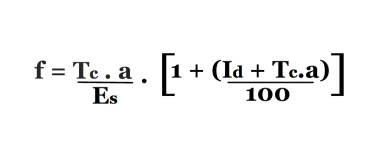
\includegraphics{Clipboard-Image.png width=383px height=151px}

Sendo: f = fator previdenciário; Es = expectativa de sobrevida no
momento da aposentadoria; Tc = tempo de contribuição até o momento da
aposentadoria; Id = idade no momento da aposentadoria; a = alíquota de
contribuição correspondente a 0,31.

\hypertarget{regra-da-idade-muxednima-caruxeancia-art.-18}{%
\subsubsection{Regra da idade mínima + carência (art.
18)}\label{regra-da-idade-muxednima-caruxeancia-art.-18}}

O art. 18 da EC 103/2019 assegura a aposentadoria daqueles filiados ao
RGPS até 13/11/2019, que cumpram as seguintes condições:

a) 60 anos de idade, se mulher e 65 anos de idade, se homem e

b) 15 anos de contribuição, para ambos os sexos. Essa regra, porém,
possui idade mínima progressiva (somente para as mulheres), a partir de
janeiro de 2020, aumentando em seis meses a cada ano, até alcançar 62,
na forma abaixo:

\begin{longtable}[]{@{}
  >{\raggedright\arraybackslash}p{(\columnwidth - 4\tabcolsep) * \real{0.5362}}
  >{\raggedright\arraybackslash}p{(\columnwidth - 4\tabcolsep) * \real{0.3333}}
  >{\raggedright\arraybackslash}p{(\columnwidth - 4\tabcolsep) * \real{0.1304}}@{}}
\toprule\noalign{}
\begin{minipage}[b]{\linewidth}\raggedright
\emph{Ano de cumprimento dos requisitos}
\end{minipage} & \begin{minipage}[b]{\linewidth}\raggedright
\emph{Idade mínima (anos)}
\end{minipage} & \begin{minipage}[b]{\linewidth}\raggedright
\end{minipage} \\
\midrule\noalign{}
\endhead
\bottomrule\noalign{}
\endlastfoot
\emph{Ano de cumprimento dos requisitos} & \emph{Mulher} &
\emph{Homem} \\
Até 31/12/2019 & 60 & 65 \\
2020 & 60,5 & 65 \\
2021 & 61 & 65 \\
2022 & 61,5 & 65 \\
A partir de 2023 & 62 & 65 \\
\end{longtable}

\hypertarget{regra-da-idade-muxednima-com-peduxe1gio-art.-20}{%
\subsubsection{Regra da idade mínima com pedágio (art.
20)}\label{regra-da-idade-muxednima-com-peduxe1gio-art.-20}}

O art. 20, incisos I, II e IV, da EC 103/2019 assegura a aposentadoria
dos filiados ao RGPS até 13/11/2019\footnote{O inciso III trata apenas
  dos servidores públicos.} que cumpram os seguintes requisitos:

\begin{enumerate}
\def\labelenumi{(\roman{enumi})}
\tightlist
\item
  57 anos de idade se mulher e 60 anos de idade, se homem;
\item
  30 anos de contribuição se mulher e 35 anos de contribuição, se homem;
\item
  ``pedágio'' (período de contribuição adicional) correspondente ao
  tempo que, na data de entrada em vigor da EC 103/2019, faltaria para
  atingir o tempo mínimo de contribuição de 30 anos (mulher) ou 35 anos
  (homem).
\end{enumerate}

Em resumo:

\begin{longtable}[]{@{}
  >{\raggedright\arraybackslash}p{(\columnwidth - 8\tabcolsep) * \real{0.0796}}
  >{\raggedright\arraybackslash}p{(\columnwidth - 8\tabcolsep) * \real{0.0448}}
  >{\raggedright\arraybackslash}p{(\columnwidth - 8\tabcolsep) * \real{0.1244}}
  >{\raggedright\arraybackslash}p{(\columnwidth - 8\tabcolsep) * \real{0.0448}}
  >{\raggedright\arraybackslash}p{(\columnwidth - 8\tabcolsep) * \real{0.7065}}@{}}
\toprule\noalign{}
\begin{minipage}[b]{\linewidth}\raggedright
\emph{Idade Mínima}
\end{minipage} & \begin{minipage}[b]{\linewidth}\raggedright
\end{minipage} & \begin{minipage}[b]{\linewidth}\raggedright
\emph{Tempo de contribuição}
\end{minipage} & \begin{minipage}[b]{\linewidth}\raggedright
\end{minipage} & \begin{minipage}[b]{\linewidth}\raggedright
``Pedágio''
\end{minipage} \\
\midrule\noalign{}
\endhead
\bottomrule\noalign{}
\endlastfoot
\emph{Mulher} & \emph{Homem} & \emph{Mulher} & \emph{Homem} & 100\% do
tempo de contribuição que, em 13/11/2019, faltava para completar 30 anos
de contribuição (mulher) ou 35 anos de contribuição (homem) \\
57 & 60 & 30 & 35 & 100\% do tempo de contribuição que, em 13/11/2019,
faltava para completar 30 anos de contribuição (mulher) ou 35 anos de
contribuição (homem) \\
\end{longtable}

Nesta regra, há uma redução, em 05 anos na idade e no tempo de
contribuição mínima para os professores da educação infantil, ensino
fundamental e médio (§ 1º). O valor da RMI da aposentadoria concedida
com base no art. 20 da EC 103/2019 corresponderá a 100\% do salário de
benefício até que lei disciplina o cálculo dos benefícios do RGPS (EC
103/2019, art. 20, § 2º, II, c/c o art. 26, § 3º, I).

Abaixo, fazemos um resumo das regras de transição, indicando o
fundamento legal de cada uma delas e dos segurados que, possivelmente,
se beneficiariam de cada uma delas:



\end{document}
